\documentclass[tikz,border=10pt]{standalone}
\usepackage{tikz}
\usepackage{amsmath,amssymb}
\usetikzlibrary{automata,backgrounds,shapes,arrows,positioning,calc,fit}

% Custom commands
\newcommand{\push}[1][]{\mathsf{push}_{#1}}
\newcommand{\pop}[1][]{\mathsf{pop}_{#1}}
\newcommand{\done}{\mathsf{done}}

\begin{document}
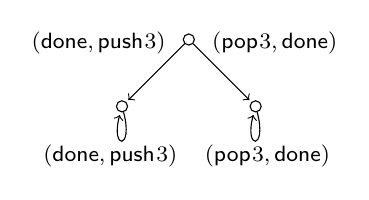
\begin{tikzpicture}[state/.style={draw,ellipse}, shorten >=1pt, node distance=2cm, on grid, auto,every node/.style={font=\footnotesize},inner sep=.05cm,node distance=1.2cm]
  % States for the \pop{3}^*;\push{3}^*
  % \node[state] (q1) at (1,0) {$$};
  \node[state] (q2) {};
  \node[state] (q3) [below left=of q2] {};
  \node[state] (q4) [below right=of q2] {};

  % Arrows for the \pop{3}^*;\push{3}^*
  \path[->]
    (q2) edge node [swap, near start] {$(\done,\push{3})$} (q3)
    % (q2) edge[loop  right] node {$(\pop{3},\push{3})$} ()
    (q3) edge[loop  below, swap] node[swap] {$(\done,\push{3})\quad$} ()
    (q2) edge node [near start] {$(\pop{3},\done)$} (q4)
    (q4) edge[loop  below] node {\quad$(\pop{3},\done)$} ();
\end{tikzpicture}
\end{document}